\chapter{Quadrilatères}\label{ChQuadrilateres}

\begin{acquis} % enlever le lien internet
\begin{itemize}
\item citer les définitions d'un parallélogramme, d'un losange, d'un rectangle et d'un carré;
\item utiliser les propriétés des différents quadrilatères, en particulier celles de leurs diagonales;
\item tracer des quadrilatères particuliers à partir de leurs propriétés.
\end{itemize}
\end{acquis}

\activites

\input{Quadrilateres/Quadrilateres_acti.tex}

\cours
\prof
{Les exercices rituels de ce chapitre porteront sur les notations.\\
\newline

Voici un lien permettant de trouver le jeu \href{http://jeux2maths.fr/tripoly/}{TRIPOLY} sur le site de jeux2maths.fr. Il s'agit de lire les codages sans se fier au visuel et d'en déduire la nature d'une figure. Attention: ce jeu contient des cerfs-volants à retirer potentiellement de la partie.}


%%%%%%%%%%%%%%%%%%%%%%%%%%%%%%%%%%%%%%%%%%%%%%%%%%%%%%%%%%%%%
 
 \prof{
\begin{activite}[Jeu: "Qui est-ce?"]
\underline{Matériel:} 
Un papier avec le nom d’un élève préalablement bien choisi en secret par le professeur.\\
\underline{Mise en place:}
Pousser toutes les tables sur le côté afin de pouvoir utiliser l’espace de la classe.
Faire mettre tous les élèves au fond de la classe.\\
\underline{Consigne:}
Connaissez-vous le jeu du qui est-ce ? Il s’agit de récupérer des informations sur un personnage pour en découvrir l’identité.
Ici, on va faire la même chose. J’ai écris le prénom de l’un d’entre-vous dans ce papier (pour que vous soyez sûrs que je ne triche pas !). Je vais donner des informations à son sujet. Si vous êtes concernés, vous avancez d’un pas.
Je dois être capable de donner suffisamment d’informations utiles pour qu’à la fin il ne reste plus que la personne dont le prénom est écrit.\\
\underline{Activité:} 
Il/elle:
\begin{itemize}
    \item est élève en 6ème
    \item est un élève en 6eF...
    \item est une fille / un garçon
    \item est blond(e)
    \item porte des lunettes
    \item ...
\end{itemize}
\underline{Lien avec le chapitre:}
\begin{itemize}
    \item est-ce que toutes les \textcolor{G1}{filles} sont des \textcolor{G1}{Marie}?
    \item Est-ce que \textcolor{G1}{Marie} est une \textcolor{G1}{fille}?
    \item Est-ce que tous les \textcolor{G1}{6eF2} portent des \textcolor{G1}{lunettes}?
    \item Est-ce que tous les gens qui portent des \textcolor{G1}{lunettes} (dans cette salle) sont des \textcolor{G1}{6eF2}?
\end{itemize}
On constate que ça marche dans un sens mais pas dans l'autre.\\
\newline
Il en est de même pour les quadrilatères. Ils ont tous des caractéristiques (de propriétés) qui nous permettent de les classer en commençant par ceux qui en ont le moins jusqu’à celui qui en a le plus. A chaque étape, on ajoute une propriété qui permet de se rapprocher un petit peu plus du quadrilatère le plus complet.\\
\newline
On va essayer de faire ça pour les quadrilatères: construire la hiérarchie des quadrilatères.\\
\begin{itemize}
    \item est-ce que toutes les \textcolor{G1}{parallélogrammes} sont des \textcolor{G1}{carrés}?
    \item Est-ce que tous les \textcolor{G1}{carrés} sont des \textcolor{G1}{parallélogrammes}?
    \item Est-ce que tous les \textcolor{G1}{parallélogrammes} ont \textcolor{G1}{4 angles droits}?
    \item Est-ce que tous les quadrilatères qui ont \textcolor{G1}{4 angles droits} sont des \textcolor{G1}{rectangles}?
\end{itemize}

\end{activite}
}
 
 %%%%%%%%%%%%%%%%%%%%%%%%%%%%%%%%%%%%%%%%%%%%%%%%%%%%%%%%%%%%%

\section{Définitions des principaux quadrilatères particuliers}
RemarqueBN : j'ai placé la figure suivante ici pour voir si on en a besoin, sinon, on l'enlèvera :
\begin{tikzpicture}[every node/.style={scale=0.7}]
% définition des styles
\def\couleur{yellow!50}
\tikzstyle{quadri}=[draw,fill=\couleur,text=blue]
\tikzstyle{estun}=[->,>=latex,very thick,dotted]

%%%%% les nœuds %%%%%
%%%Quadrilatère
\node (Q) at (0,2) {Quadrilatère};
\coordinate[shift={(0mm,1mm)}] (Q1) at (Q.north west);
\coordinate[shift={(2mm,-1mm)}] (Q2) at (Q.north east);
\coordinate[shift={(-3mm,1mm)}] (Q3) at (Q.south east);
\coordinate[shift={(2mm,-2mm)}] (Q4) at (Q.south west);
\draw[fill=\couleur] (Q1)--(Q2)--(Q3)--(Q4)--cycle;
\node[blue] (Q) at (0,2) {Quadrilatère};
%%%Parallélogramme
\node[rectangle] (P) at (0,1) {Parallélogramme};
\coordinate[shift={(-3mm,0mm)}] (P1) at (P.north west);
\coordinate[shift={(-3mm,0mm)}] (P2) at (P.north east);
\coordinate[shift={(3mm,0mm)}] (P3) at (P.south east);
\coordinate[shift={(3mm,0mm)}] (P4) at (P.south west);
\draw[fill=\couleur] (P1)--(P2)--(P3)--(P4)--cycle;
\node[color=blue] (P) at (0,1) {Parallélogramme};
%%%Rectangle
\node[rectangle,quadri] (R) at (-1,0) {Rectangle};
%%%Losange
\node[shape=diamond,shape aspect=2,quadri] (L) at (1.5,0) {Losange};
%%%Carré
\node[quadri,minimum size=1.2cm] (C) at (0,-1) {Carré};
%%%Trapèze
\node (T) at (2,2) {Trapèze};
\coordinate[shift={(0mm,0mm)}] (T1) at (T.north west);
\coordinate[shift={(0mm,0mm)}] (T2) at (T.north east);
\coordinate[shift={(4mm,0mm)}] (T3) at (T.south east);
\coordinate[shift={(-2mm,0mm)}] (T4) at (T.south west);
\draw[fill=\couleur] (T1)--(T2)--(T3)--(T4)--cycle;
\node[blue] (T) at (2,2) {Trapèze};

%%%%% les flèches %%%%%
\draw[estun] (P)--(Q);
\draw[estun] (R.north)--(P);
\draw[estun] (L.north west)--(P);
\draw[estun] (C)--(R.south);
\draw[estun] (C)--(L.south west);
\coordinate[shift={(-1mm,0mm)}] (TFl) at (T.west);
\draw[estun] (TFl)--(Q);

%%%%%% la légende %%%%%
\draw[estun] (1,-1.2)--(2.3,-1.2)node[midway,above]{est un};
\end{tikzpicture}
\begin{definition}
Le \MotDefinition{quadrilatère}{} :
Un quadrilatère est un polygone (figure qui a plusieurs côtés) qui possède 4 côtés. Il est dit quelconque quand il ne possède aucune autre propriété (il n'a rien de particulier).\\
Il a donc 4 sommets et 4 angles.\\


\begin{minipage}[t]{0.50\linewidth}
\begin{center} \textbf{Quadrilatère convexe}\\
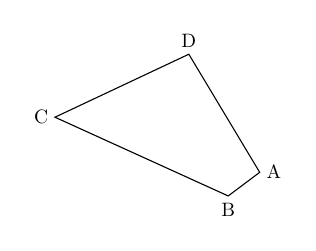
\begin{tikzpicture}[every node/.style={scale=0.7}]
    \draw (0,0) node[left]{C}--(1.7,0.8) node[above]{D}--(2.6,-0.7)node[right]{A}--(2.2,-1)node[below]{B}--cycle;
\end{tikzpicture}
\end{center}
\end{minipage}
\begin{minipage}[t]{0.50\linewidth}
\begin{center}\textbf{Quadrilatère concave}\\
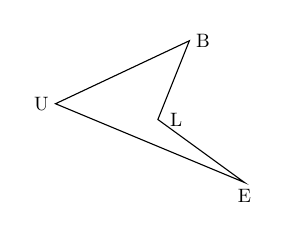
\begin{tikzpicture}[every node/.style={scale=0.7}]
    \draw (0,0) node[left]{U}--(1.7,0.8) node[right]{B}--(1.3,-0.2)node[right=1mm]{L}--(2.4,-1)node[below]{E}--cycle;
\end{tikzpicture}
\end{center}
\end{minipage}
\end{definition}

Deux côtés qui possèdent un sommet commun sont appelés 
\textcolor{B2}{sommets consécutifs}. De même, deux sommets liés par un côté sont dits \textcolor{B2}{consécutifs}.\\
Deux sommets ou deux côtés non consécutifs d'un quadrilatère sont des \textcolor{B2}{sommets opposés} ou \textcolor{B2}{côtés opposés}.\\
Les segments qui joignent deux sommets non consécutifs d'un quadrilatère sont appelés \textcolor{B2}{les diagonales} du quadrilatère.
\begin{center}
   \begin{tikzpicture}[every node/.style={scale=0.6}]

%pour le tracé
%\draw[gray!30] (-5,-5) grid (5,5);
%\fill[red] (0,0) circle (3pt);

% définition des styles
\def\couleur{yellow!50}
\tikzstyle{quadri}=[draw,fill=\couleur,text=blue]

%carré
\begin{scope}[xshift=1.6cm,yshift=-0.2cm,scale=0.8,rotate=-10] 
\draw (0,0)--(1,0)--(1,1)--(0,1)--cycle;
%\draw (0.1,0)|-(0,0.1);
\end{scope}

%carré avec 4 côtés égaux
%\begin{scope}[xshift=1.8cm,yshift=-1cm,scale=0.8,rotate=10] 
%\draw (0,0)--(1,0)--(1,1)--(0,1)--cycle;
%\node at (0.5,0) {$\times$};
%\node at (1,0.5) {$\times$};
%\node at (0,0.5) {$\times$};
%\node at (0.5,1) {$\times$};
%\end{scope}

%losange avec 4 côtés égaux
\begin{scope}[xshift=3.8cm,yshift=0.8cm,rotate=-20] 
\draw (0,0)--(0.6,1)--(1.2,0)--(0.6,-1)--cycle;
\node at (0.3,0.5) {$\circ$};
\node at (0.9,0.5) {$\circ$};
\node at (0.9,-0.5) {$\circ$};
\node at (0.3,-0.5) {$\circ$};
\end{scope}

%losange avec diagonales perpendiculaires
\begin{scope}[xshift=5.3cm,yshift=-0.4cm,rotate=-45] 
\draw (0,0)--(0.6,1)--(1.2,0)--(0.6,-1)--cycle;
\draw (0,0)--(1.2,0);
\draw (0.6,1)--(0.6,-1);
\draw (0.7,0)|-(0.6,0.1);
\end{scope}

%rectangle avec 1 angle droit
\begin{scope}[xshift=-1.1cm,yshift=0.7cm,rotate=-15] 
\draw (0,0)--(0,.8)--(1.5,.8)--(1.5,0)--cycle;
\draw (0.1,0)|-(0,0.1);
\end{scope}

%rectangle avec diagonales de même longueur
\begin{scope}[xshift=-2.3cm,yshift=-1.2cm,rotate=40] 
\draw (0,0)--(0,.8)--(1.6,.8)--(1.6,0)--cycle;
\draw (0,0)--(1.6,0.8);
\draw (0,.8)--(1.6,0);
\node at (0.4,0.2) {$\circ$};
\node at (1.2,0.2) {$\circ$};
\node at (0.4,0.6) {$\circ$};
\node at (1.2,0.6) {$\circ$};
\end{scope}

%parallélogramme avec diagonales se coupant au milieu
\begin{scope}[xshift=-0.6cm,yshift=2.4cm,rotate=-10] 
\draw (0,0)--(0.4,.8)--(2,.8)--(1.6,0)--cycle;
\draw (0,0)--(2,0.8);
\draw (0.4,.8)--(1.6,0);
\node at (0.5,0.2) {$\circ$};
\node at (1.5,0.6) {$\circ$};
\node[rotate=50] at (0.7,0.6) {$\times$};
\node[rotate=50] at (1.3,0.2) {$\times$};
\end{scope}

%parallélogramme avec côtés opposés égaux
\begin{scope}[xshift=2.2cm,yshift=2cm,rotate=10] 
\draw (0,0)--(0.4,0.8)--(2,0.8)--(1.6,0)--cycle;
\node at (0.2,0.4) {$\circ$};
\node at (1.8,0.4) {$\circ$};
\node[rotate=0] at (1.2,0.8) {$\times$};
\node[rotate=0] at (0.8,0) {$\times$};
\end{scope}


%parallélogramme avec angles opposés égaux
\begin{scope}[xshift=1.5cm,yshift=-3cm,rotate=0] 
\draw (0,0)--(0.4,0.8)--(2,0.8)--(1.6,0)--cycle;
\end{scope}

%quadrilatère quelconque
\begin{scope}[xshift=5.8cm,yshift=-3cm,rotate=0] 
\draw (0,0)--(1,0.7)--(1.2,-0.15)--(0.5,-0.3)--cycle;
\end{scope}

%trapèze 1
\begin{scope}[xshift=-4.8cm,yshift=1.5cm,scale=0.8,rotate=20] 
\draw (0,0)--(0.8,0.6)--(1.8,0.6)--(2,0)--cycle;
\end{scope}

%trapèze 2
\begin{scope}[xshift=-4.8cm,yshift=1cm,scale=0.9,rotate=-20] 
\draw (0,0)--(0.1,0.4)--(0.7,0.4)--(1,0)--cycle;
\end{scope}

%cerf-volant avec diagonales perpendiculaires et côtés consécutifs égaux
\begin{scope}[xshift=7.6cm,yshift=1.5cm,rotate=10] 
\draw (0,0)--(0.5,0.6)--(1,0)--(0.5,-1.2)--cycle;
\draw (0,0)--(1,0);
\draw (0.5,0.6)--(0.5,-1.2);
\draw (0.6,0)|-(0.5,0.1);
\node[rotate=40] at (0.25,0.3) {$\times$};
\node[rotate=40] at (0.75,0.3) {$\times$};
\node[rotate=0] at (0.75,-0.6) {$\circ$};
\node[rotate=0] at (0.25,-0.6) {$\circ$};
\end{scope}


%%%%%%%% Éllipes des ensembles
\begin{scope}[xshift=0cm,yshift=0cm,rotate=0] 

%\tikzset{ellipse1/.pic={\draw [xscale=0.8,ultra thick,color=green] (0,0) circle (2);}}
%\tikzset{ellipse2/.pic={\draw [xscale=0.8,ultra thick,color=red] (0,0) circle (2);}}
%\pic at (5,0) {ellipse1};
%\pic at (6,0) {ellipse2};

\begin{scope} %coloration de la zone des carrés
\clip [xscale=1.6,yscale=1] (0,0) circle (2);
\fill[xscale=1.6,yscale=1,color=A3,opacity=0.3] (2.5,0) circle (2); 
\end{scope}

\draw[xscale=1.6,yscale=1,ultra thick,color=H2] (0,0) circle (2);
\draw[xscale=1.6,yscale=1,ultra thick, color=B2] (2.5,0) circle (2);
\draw[xscale=1.6,yscale=1,ultra thick, color=J2] (1.3,0) circle (3.5);
\draw[xscale=1.95,yscale=1.2,ultra thick, color=F2] (1,0) circle (4);
\end{scope}


%elipse autour des trapèzes
\node[draw,ultra thick, color=C1,shape=ellipse,minimum width=4cm,minimum height=3cm,rotate=50] (A) at (-4.2,1.5) {};
\node[text width=2cm,text centered] (B) at (-6,3){trapèzes : deux côtés opposés parallèles};
\draw (B) to [out=-90,in=90] (A);
\end{tikzpicture}
\end{center}

\begin{definition}
Le \MotDefinition{trapèze}{} est un quadrilatère dont \textcolor{C2}{\textbf{deux côtés opposés sont parallèles}}. \\
 \begin{center}
  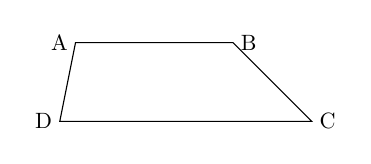
\begin{tikzpicture}[rotate=0,every node/.style={scale=0.8}]
  \draw (-1,0) node[left]{A} -- (1,0) node[right]{B} -- (2,-1)node[right]{C} -- (-1.2,-1) node[left]{D} -- cycle;
\end{tikzpicture}
\end{center}

Les côtés parallèles du trapèze sont appelés \textcolor{C2}{\textbf{bases du trapèze}}.
\end{definition}

\begin{definition}
Le \MotDefinition{parallélogramme}{} est un quadrilatère dont les côtés opposés sont \textcolor{C2}{\textbf{parallèles deux à deux}}. \\
  \begin{center}
  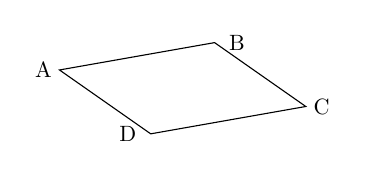
\begin{tikzpicture}[rotate=10,every node/.style={scale=0.8}]
  \draw (-1,0) node[left]{A} -- (1,0) node[right=3pt]{B} -- (2,-1)node[right]{C} -- (0,-1) node[left=3pt]{D} -- cycle;
\end{tikzpicture}
\end{center}
\end{definition}

 
\begin{minipage}[t]{0.49\linewidth}
  \begin{definition}
   Le \MotDefinition{rectangle}{} est un parallélogramme qui a \textcolor{C2}{\textbf{1 angle droit}}.
  
\begin{center}
\begin{tikzpicture}[rotate=0,every node/.style={scale=0.8}]
\draw (-1,0) node[left]{A} -- (1,0) node[right]{B} -- (1,-1)node[right]{C} -- (-1,-1) node[left]{D} -- cycle;
\draw[very thick,color=C2] (-1,-0.2)-|(-0.8,0);
\end{tikzpicture}
\end{center}
 \end{definition}
 \end{minipage}
 %
 \begin{minipage}[t]{0.59\linewidth}
   \begin{definition}
   Le \MotDefinition{losange}{} un parallélogramme qui a \textcolor{C2}{\textbf{2 côtés consécutifs de même longueur}}.
   
\begin{center}
\begin{tikzpicture}[rotate=0,every node/.style={scale=0.8}]
\draw (-0.7,0) node[left]{A} -- (0,1) node[above]{B} -- (0.7,0)node[right]{C} -- (0,-1) node[below]{D} -- cycle;
\node[color=C2,rotate=45] at (-.35,.5){$\times$};
\node[color=C2,rotate=-45] at (.35,.5){$\times$};
%\node[color=C2,rotate=45] at (.35,-.5){$\times$};
%\node[color=C2,rotate=-45] at (-.35,-.5){$\times$};
\end{tikzpicture}
\end{center}
   \end{definition}
  \end{minipage} 
  
\begin{definition}
Le \MotDefinition{carré}{} est un parallélogramme qui a les propriétés du rectangle et du losange. \\

\begin{center}
\begin{tikzpicture}[rotate=0,every node/.style={scale=0.8}]
\draw (0,0) node[left]{A} -- (1,0) node[right]{B} -- (1,-1)node[right]{C} -- (0,-1) node[left]{D} -- cycle;
\draw[very thick,color=C2] (0,-0.2)-|(0.2,0);
\node[color=C2] at (.5,0){$\times$};
\node[color=C2] at (1,-.5){$\times$};
%\node[color=C2] at (.5,-1){$\times$};
%\node[color=C2] at (0,-.5){$\times$};
\end{tikzpicture}
\end{center}
\end{definition}

\section{Propriétés des principaux quadrilatères particuliers}

\begin{tikzpicture}
% définition des styles
\def\couleur{H4!50}
\def\echellequadri{1.2}
\def\echelleppte{0.8}
\tikzstyle{quadri}=[draw,color=H1,fill=\couleur,text=H1,scale=\echellequadri]
\tikzstyle{txtpptecote}=[text=A1,scale=\echelleppte,fill=white,text width=2cm,text badly centered]
\tikzstyle{txtpptediag}=[text=B2,scale=\echelleppte,fill=white,text width=2cm,text badly centered]
\tikzstyle{lignepptecote}=[->,>=latex,very thick,dotted,color=A1]
\tikzstyle{lignepptediag}=[->,>=latex,very thick,dotted,color=B2]


%%%%% les nœuds %%%%%
%%%Parallélogramme
\node[scale=\echellequadri] (P) at (0,4) {Parallélogramme};
\coordinate[shift={(-2mm,0mm)}] (P1) at (P.north west);
\coordinate[shift={(-2mm,0mm)}] (P2) at (P.north east);
\coordinate[shift={(2mm,0mm)}] (P3) at (P.south east);
\coordinate[shift={(2mm,0mm)}] (P4) at (P.south west);
\draw[color=H1,fill=\couleur] (P1)--(P2)--(P3)--(P4)--cycle;
\node[color=H1,scale=\echellequadri] (P) at (0,4) {Parallélogramme};
%%%Rectangle
\node[rectangle,quadri] (R) at (-3.2,0) {Rectangle};
%%%Losange
\node[shape=diamond,shape aspect=2,quadri] (L) at (4.2,0) {Losange};
%%%Carré
\node[quadri,minimum size=1.2cm] (C) at (0,-4) {Carré};

%%%%% les flèches avec le texte %%%%%
\draw[lignepptecote] (P) .. controls +(175:4cm) and +(160:4cm)..(R) node[txtpptecote,pos=0.7]{avec 2 côtés consécutifs perpendiculaires};

\draw[lignepptediag] (P) .. controls +(180:4cm) and +(90:0.6cm)..(R)node[txtpptediag,pos=0.6]{avec diagonales de même longueur};

\draw[lignepptecote] (P) .. controls +(10:4cm) and +(50:4cm)..(L)node[txtpptecote,pos=0.8]{avec 2 côtés consécutifs égaux};

\draw[lignepptediag] (P) .. controls +(0:3cm) and +(100:3cm)..(L)node[txtpptediag,pos=0.6]{avec diagonales perpendiculaires};

\draw[lignepptecote] (R) .. controls +(-130:4cm) and +(-160:4cm)..(C)node[txtpptecote,pos=0.4]{avec 2 côtés consécutifs égaux};

\draw[lignepptediag] (R) .. controls +(-70:3cm) and +(160:2cm)..(C)node[txtpptediag,pos=0.4]{avec diagonales perpendiculaires};

\draw[lignepptecote] (L) .. controls +(-50:3cm) and +(-20:3cm)..(C)node[txtpptecote,pos=0.4]{avec 2 côtés consécutifs perpendiculaires};

\draw[lignepptediag] (L) .. controls +(-110:3cm) and +(20:2cm)..(C)node[txtpptediag,pos=0.5]{avec diagonales de même longueur};

\end{tikzpicture}

\section{Méthodes de construction}

\begin{methode*1}[Construire un parallélogramme avec la règle et l'équerre]

\vspace{0.8em}
\textcolor{H1}{\textbf{Remarque}} : On utilise ici le fait que les côtés opposés sont parallèles deux à deux.

\begin{exemple*1}
Soient trois points $A$, $B$ et $C$ non alignés. Place le point $D$ tel que $ABCD$ soit un parallélogramme.\\[0.5em]


\begin{tabularx}{\textwidth}{X|X|X}
   \qquad \input{./Quadrilateres/figures/Parallelo_RegleEquerre_1} & \input{./Quadrilateres/figures/Parallelo_RegleEquerre_2} & 
\begin{tikzpicture}[every node/.style={scale=0.7}]
\draw[dashed](-0.8,0)--(1.2,0);
\draw[dashed](-0.8,1.2)--(1,1.2);
\draw[dashed](-0.92,1.39)--(.16,-0.23);
\draw[dashed](0.08,1.39)--(1.15,-.22);
\draw[thick,H1,densely dashed,->,>=stealth](.43,0.85)--(-0.26,0.39); 

\draw[thick] (0,0) node{$\times$} -- (1,0) node{$\times$} -- (0.2,1.2)node{$\times$};
\node[below right] at (0,0){A};
\node[below right] at (1,0){B};
\node[above right] at (0.2,1.2){C};
\node[above right] at (-0.8,1.2){D};
\node at (-0.8,1.2){$\times$};

%%%%%%%%%%%%%%%%%%%%%%%%
%%%%%%%%%%%%%%%%%%%%%%%%
%Début règle !! Si la figure est tournée, il faut
%rajouter l'angle de rotation dans le node des graduation
%pour que les nombres soient écrits correctement
%%%%%%%%%%%%%%%%%%%%%%%%
%%%%%%%%%%%%%%%%%%%%%%%% 

    %Graduation max. de la règle
    \def \Taille {6}
    %Définition de l 'angle de rotation de la règle
    \def \Rotation {-90-56.31}
    %Définition du décalage de la règle
    \def \DecalX {0.7}
    \def \DecalY {1.6}
    %Couleur des élèments de la règle (sauf le remplissage)
    \def \RegleColor {blue!60}

\begin{scope}[shift={(\DecalX,\DecalY)},rotate=\Rotation,scale=.35]
    % contours de la règle
    \draw[color=\RegleColor, fill =blue!5, opacity=0.5,rounded corners=2pt] (-0.2,0.5) rectangle (\Taille+0.2,-0.5);	%Dont couleur de remplissage
    % graduation 1 mm
    \foreach \a in {0,0.1,...,\Taille}{\draw[color=\RegleColor] (\a,0.5)--(\a,0.42);}
    % graduation 5 mm
    \foreach \a in {0,0.5,...,\Taille}{\draw[color=\RegleColor] (\a,0.42)--(\a,0.35);}
    % graduation et repères 10 mm
    \foreach \a in {0,1,...,\Taille}{\draw[color=\RegleColor] (\a,0.35)--(\a,0.25);}
\end{scope}

%%%%%%%%%%%%%%%%%%%%%%%%
%%%%%%%%%%%%%%%%%%%%%%%%
%Fin de la règle
%%%%%%%%%%%%%%%%%%%%%%%%
%%%%%%%%%%%%%%%%%%%%%%%%

%%%%%%%%%%%%%%%%%%%%%%%%
%%%%%%%%%%%%%%%%%%%%%%%%
%Définition des paramètres de l'équerre
%et de son positionnement
%%%%%%%%%%%%%%%%%%%%%%%%
%%%%%%%%%%%%%%%%%%%%%%%%

\def \xorigine {0.25}; %abscisse de l'origine de l'équerre posée avec un xshift
\def \yorigine {1.08}; %ordonnée de l'origine de l'équerre posée avec un yshift
\def \rotation {-90-56.31}; %angle de rotation de l'équerre
\def \longueur {4}; %longueur de l'équerre
\def \largeur {2}; %largeur de l'équerre
\def \epaisseur {\longueur * 0.1}; %épaisseur de la partie «colorée» de l'équerre

%%%%%%%%%%%%%%%%%%%%%%%%
%%%%%%%%%%%%%%%%%%%%%%%%
%Tracé de l'équerre
%%%%%%%%%%%%%%%%%%%%%%%%
%%%%%%%%%%%%%%%%%%%%%%%%

\begin{scope}[xshift=\xorigine cm,yshift=\yorigine cm,rotate=\rotation,scale=0.25]

%contour extérieur de l'équerre
\coordinate (A) at (0,0) ; %«origine» de l'équerre
\coordinate (B) at (\largeur,0) ;
\coordinate (C) at (0,\longueur) ;
\draw [gray](A)--(B)--(C)--cycle;


%contour intérieur de l'équerre
\coordinate (D) at (\epaisseur,\epaisseur) ;
\coordinate (E) at ($\largeur*(1,0)-{\largeur * \epaisseur / \longueur}*(1,0)-\epaisseur*(1,0)+\epaisseur*(0,1)$);
\coordinate (F) at ($\epaisseur*(1,0)+\longueur*(0,1)-{2*\longueur * \epaisseur / \largeur}*(0,1)$);
\draw [gray](D)--(E)--(F)--cycle;

%partie colorée de l'équerre
\fill [color=blue!50!gray,opacity=.4,even odd rule] (A)--(B)--(C)--cycle (D)--(E)--(F)--cycle;%l'option even odd rule permet de faire le remplissage entre les 2 zones définies

\end{scope}
%%%%%%%%%%%%%%%%%%%%%%%%
%%%%%%%%%%%%%%%%%%%%%%%%
%Fin de l'équerre
%%%%%%%%%%%%%%%%%%%%%%%%
%%%%%%%%%%%%%%%%%%%%%%%%

%%%%%%%%%%%%%%%%%%%%%%%%
%%%%%%%%%%%%%%%%%%%%%%%%
%Définition des paramètres de l'équerre
%et de son positionnement
%%%%%%%%%%%%%%%%%%%%%%%%
%%%%%%%%%%%%%%%%%%%%%%%%

\def \xorigine {-0.43}; %abscisse de l'origine de l'équerre posée avec un xshift
\def \yorigine {0.63}; %ordonnée de l'origine de l'équerre posée avec un yshift
\def \rotation {-90-56.31}; %angle de rotation de l'équerre
\def \longueur {4}; %longueur de l'équerre
\def \largeur {2}; %largeur de l'équerre
\def \epaisseur {\longueur * 0.1}; %épaisseur de la partie «colorée» de l'équerre

%%%%%%%%%%%%%%%%%%%%%%%%
%%%%%%%%%%%%%%%%%%%%%%%%
%Tracé de l'équerre
%%%%%%%%%%%%%%%%%%%%%%%%
%%%%%%%%%%%%%%%%%%%%%%%%

\begin{scope}[xshift=\xorigine cm,yshift=\yorigine cm,rotate=\rotation,scale=0.25]

%contour extérieur de l'équerre
\coordinate (A) at (0,0) ; %«origine» de l'équerre
\coordinate (B) at (\largeur,0) ;
\coordinate (C) at (0,\longueur) ;
\draw [gray](A)--(B)--(C)--cycle;


%contour intérieur de l'équerre
\coordinate (D) at (\epaisseur,\epaisseur) ;
\coordinate (E) at ($\largeur*(1,0)-{\largeur * \epaisseur / \longueur}*(1,0)-\epaisseur*(1,0)+\epaisseur*(0,1)$);
\coordinate (F) at ($\epaisseur*(1,0)+\longueur*(0,1)-{2*\longueur * \epaisseur / \largeur}*(0,1)$);
\draw [gray](D)--(E)--(F)--cycle;

%partie colorée de l'équerre
\fill [color=blue!50!gray,opacity=.4,even odd rule] (A)--(B)--(C)--cycle (D)--(E)--(F)--cycle;%l'option even odd rule permet de faire le remplissage entre les 2 zones définies

\end{scope}
%%%%%%%%%%%%%%%%%%%%%%%%
%%%%%%%%%%%%%%%%%%%%%%%%
%Fin de l'équerre
%%%%%%%%%%%%%%%%%%%%%%%%
%%%%%%%%%%%%%%%%%%%%%%%%

%%%%%%%%%%%%%%%%%%%%%%%%
%%%%%%%%%%%%%%%%%%%%%%%%
%Début crayon
%%%%%%%%%%%%%%%%%%%%%%%%
%%%%%%%%%%%%%%%%%%%%%%%%

\begin{scope}[xshift=-0cm,yshift=0cm,rotate=-20,scale=.15] %le crayon, xshift et yshift pour les coordonnées de la pointe, rotate pour l'orientation du crayon
\def \couleur {black}
\coordinate (O) at (0,0);
\fill[\couleur!40] (-0.2,4.8) -- (0.2,4.8) -- (0.2,0.8) --(0.1,0.65) -- (0,0.8) -- (-0.1,0.66) -- (-0.2,0.8) -- cycle; %corps du crayon
\draw[color=white] (0,4.8) -- (0,0.8); %trait intérieur du crayon
\fill[\couleur!90] (-0.2,4.3) -- (0,4.27) -- (0.2,4.3) -- (0.2,4.8) arc(30:150:0.23cm); %partie haute du crayon
\fill[brown!40] (-0.2,0.8) -- (O)node[coordinate,pos=0.75](a){} -- (0.2,0.8)node[coordinate,pos=0.25](b){} -- (0.1,0.65) -- (0,0.8) -- (-0.1,0.66) -- cycle; %pointe du crayon (partie taillée)
\fill[\couleur!90] (a) -- (O) -- (b) -- cycle; %mine du crayon
\end{scope}

%%%%%%%%%%%%%%%%%%%%%%%%
%%%%%%%%%%%%%%%%%%%%%%%%
%Fin crayon
%%%%%%%%%%%%%%%%%%%%%%%%
%%%%%%%%%%%%%%%%%%%%%%%%

\end{tikzpicture} \\ 
 
 
 On trace les côtés $[AB]$ et $[BC]$ du quadrilatère $ABCD$. Le quadrilatère $ABCD$ est un parallélogramme, donc ses côtés opposés sont parallèles deux à deux : soit $(AB) \parallel (CD)$. & On trace la parallèle à $(AB)$ passant par $C$. & On trace la parallèle à $(BC)$ passant par $A$. Ces deux droites sont sécantes en $D$.
 
 Ainsi $ABCD$ a ses côtés opposés parallèles deux à deux, c'est donc bien un parallélogramme. \\
\end{tabularx} \\[1em]

\end{exemple*1}

\exercice
Réalise un croquis avant de construire le parallélogramme $PRLG$ tel que $PR = 5$ cm, $PG = 6$ cm et  $\widehat{RPG} = 74^\circ$ en utilisant la propriété sur le parallélisme des côtés opposés du parallélogramme.
%\correction

\end{methode*1}

\newpage





\begin{methode*1}[Construire un parallélogramme avec le compas]

 
\vspace{0.8em}
\textcolor{H1}{\textbf{Remarque}} : On utilise ici le fait que les côtés opposés d'un parallélogramme sont égaux deux à deux.

 \begin{exemple*1}
 
  \begin{tabularx}{\textwidth}{X|X|X}
   \qquad 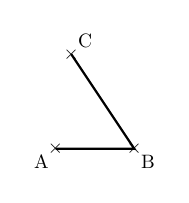
\begin{tikzpicture}[every node/.style={scale=0.7}]
\draw [thick](0,0) node{$\times$} -- (1,0) node{$\times$} -- (0.2,1.2)node{$\times$};
\node[below left] at (0,0){A};
\node[below right] at (1,0){B};
\node[above right] at (0.2,1.2){C};

\end{tikzpicture} &   \qquad 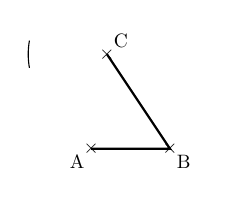
\begin{tikzpicture}[every node/.style={scale=0.7}]

\draw [thick](0,0) node{$\times$} -- (1,0) node{$\times$} -- (0.2,1.2)node{$\times$};
\node[below left] at (0,0){A};
\node[below right] at (1,0){B};
\node[above right] at (0.2,1.2){C};

\draw (-0.8,1.2) arc (180:170:1);
\draw (-0.8,1.2) arc (180:190:1);

\coordinate (C) at (0.2,1.2);
\coordinate (D) at (-0.8,1.2);
\begin{scope}[scale=0.2]
\Compas {C}{D} 
\end{scope}
\end{tikzpicture} &   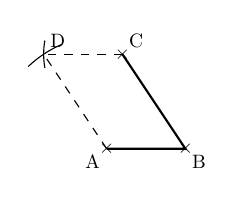
\begin{tikzpicture}[every node/.style={scale=0.7}]

\draw [thick](0,0) node{$\times$} -- (1,0) node{$\times$} -- (0.2,1.2)node{$\times$};
\node[below left] at (0,0){A};
\node[below right] at (1,0){B};
\node[above right] at (0.2,1.2){C};
\node[above right] at (-0.8,1.2){D};

\draw[dashed](0,0)--(-0.8,1.2);
\draw[dashed](0.2,1.2)--(-0.8,1.2);

\draw (-0.8,1.2) arc (180:170:1);
\draw (-0.8,1.2) arc (180:190:1);
\draw (-0.8,1.2) arc (123.69:113.69:1.44);
\draw (-0.8,1.2) arc (123.69:133.69:1.44);

\coordinate (A) at (0,0);
\coordinate (D) at (-0.8,1.2);
\begin{scope}[scale=0.2]
\Compas {A}{D} 
\end{scope}
\end{tikzpicture} \\ 
 On trace les côtés $[AB]$ et $[BC]$ du quadrilatère $ABCD$.
 
 Le quadrilatère $ABCD$ est un parallélogramme, donc ses côtés opposés $[AB]$ et $[CD]$ sont de la même longueur deux à deux : soit $AB = CD$ et $BC = AD$. & À l'aide du compas, on reporte la longueur $AB$ à partir du point $C$. & On reporte la longueur $BC$ à partir du point $A$. On place le point $D$ à l'intersection des deux arcs de cercle puis on trace les côtés $[AD]$ et $[CD]$.
 
Ainsi $ABCD$ a ses côtés opposés égaux deux à deux, c'est donc bien un parallélogramme.\\
\end{tabularx} \\
 
 \end{exemple*1}

\vspace*{1em}
Pour les deux exemples ci-dessous, faire un croquis avant de faire le tracé précis :\\[-2.5em]

\exercice
Construis le parallélogramme $DRAP$ tel que $DR = 6$ cm, $DP = 8$ cm et $\widehat{RDP} = 40^\circ$ en utilisant la propriété sur l'égalité des longueurs des côtés opposés du parallélogramme.
%\correction

\vspace{2.7cm}

\exercice
Construis un rectangle $ABCD$ tel que $AB = 3$ cm et $BC = 5$ cm.
%\correction

\end{methode*1}

%%%%%%%%%%%%%%%%%%%%%%%%%%%%%%%%%%%%%%%%%%%%%%%%%%%%%%%%%%%%

\begin{methode*1}[Construire un losange avec le compas]
 
\vspace{0.8em}
\textcolor{H1}{\textbf{Remarque}} : On utilise ici le fait qu'un losange a quatre côtés de même longueur.

\begin{exemple*1}
Construis un losange $ABCD$ de 6 cm de côté.\\[1em]
\begin{minipage}[c]{0.7\linewidth}
On fait d'abord un croquis. Dans un losange, les quatre côtés ont la même longueur. Ainsi, les triangles $ABD$ et $CBD$ sont \textbf{isocèles} respectivement en $A$ et $C$.
 \end{minipage} \hfill%
 \begin{minipage}[c]{0.24\linewidth}
  \includegraphics[width=2.6cm]{losange_croquis}
  \end{minipage} \\
  
\begin{tabularx}{\textwidth}{X|X}
\qquad 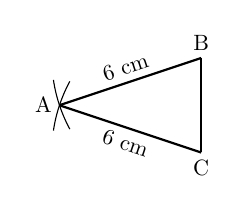
\begin{tikzpicture}[scale=1.2,every node/.style={scale=0.8}]

\draw [thick](0,0) -- (1.5,0.5) node[midway,above,sloped]{6 cm};
\draw [thick] (1.5,0.5) -- (1.5,-.5);
\draw [thick](1.5,-0.5) -- (0,0) node[midway,below,sloped]{6 cm};
\node[left] at (0,0){A};
\node[above] at (1.5,0.5){B};
\node[below] at (1.5,-0.5){C};

\draw (0,0) arc (-161.57:-151.57:1.58);
\draw (0,0) arc (-161.57:-171.57:1.58);
\draw (0,0) arc (161.57:151.57:1.58);
\draw (0,0) arc (161.57:171.57:1.58);

\coordinate (A') at (0.11,-0.25);
\coordinate (B) at (1.5,0.5);
\begin{scope}[scale=0.3]
\Compas {B}{A'} 
\end{scope}
\end{tikzpicture} & \qquad 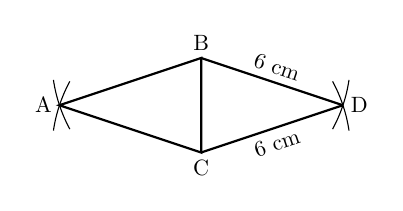
\begin{tikzpicture}[scale=1.2,every node/.style={scale=0.8}]

\draw [thick](0,0) -- (1.5,0.5) -- (1.5,-.5) -- cycle;
\draw [thick](1.5,0.5)--(3,0) node[midway,above,sloped]{6 cm};
\draw [thick](3,0) -- (1.5,-0.5) node[midway,below,sloped]{6 cm};
\node[left] at (0,0){A};
\node[above] at (1.5,0.5){B};
\node[below] at (1.5,-0.5){C};
\node[right] at (3,0){D};

\draw (0,0) arc (-161.57:-151.57:1.58);
\draw (0,0) arc (-161.57:-171.57:1.58);
\draw (0,0) arc (161.57:151.57:1.58);
\draw (0,0) arc (161.57:171.57:1.58);

\draw (3,0) arc (-161.57+180:-151.57+180:1.58);
\draw (3,0) arc (-161.57+180:-171.57+180:1.58);
\draw (3,0) arc (161.57+180:151.57+180:1.58);
\draw (3,0) arc (161.57+180:171.57+180:1.58);

\coordinate (D') at (3.06,0.27);
\coordinate (B) at (1.5,0.5);
\begin{scope}[scale=0.3]
\Compas {B}{D'} 
\end{scope}
\end{tikzpicture} \\
 On trace un segment $[BD]$. On construit un triangle $ABD$ isocèle en $A$ tel que $AB = AD = 6$ cm. & On construit le triangle $CBD$ isocèle en $C$ tel que $CB = CD = 6$ cm. \\
\end{tabularx} \\

 \end{exemple*1}

\exercice
Construis un losange $VERT$ tel que $VE = 4,5$ cm et $ET = 6,9$ cm.
%\correction

\vspace{3.5cm}

\exercice
Construis un triangle $BOL$ isocèle en $B$ tel que $BO = 2,1$ cm et $OL = 3,4$ cm. Place le point $S$ pour que $BOSL$ soit un losange.
%\correction

\end{methode*1}

%%%%%%%%%%%%%%%%%%%%%%%%%%%%%%%%%%%%%%%%%%%%%%%%%%%%%%%%%%%%



\exercicesbase
\begin{colonne*exercice}
\input{Quadrilateres/Quadrilateres_exos_entrain.tex}
\end{colonne*exercice}


\exercicesappr
\begin{colonne*exercice}
\input{Quadrilateres/Quadrilateres_exos_approf}
\end{colonne*exercice}

\connaissances

\QCMautoevaluation{Pour chaque question, plusieurs réponses sont
  proposées.  Déterminer celles qui sont correctes.}

\begin{QCM}
  \begin{GroupeQCM}
    \begin{exercice}
      Si $T$ est le milieu d'un segment $[AD]$ et que $AD = 56$ mm alors \ldots
      \begin{ChoixQCM}{4}
      \item $T \in [AD]$
      
      et $TA = 28$ mm
      \item $TA = TD$
      \item \\[-1em]
      \includegraphics[width=2.6cm]{triangleATD}
      \item $[AD]$ est un diamètre du cercle de centre $T$ et de rayon 28 mm
      \end{ChoixQCM}
\begin{corrige}
     \reponseQCM{abd} 
   \end{corrige}
    \end{exercice}

  \begin{exercice}
      Si $ROSE$ est un losange alors \ldots
      \begin{ChoixQCM}{4}
      \item $[RE]$ est une diagonale
      \item $[OS]$ est une diagonale
      \item $[OS]$ est un côté
      \item $[RS]$ est une diagonale
      \end{ChoixQCM}
\begin{corrige}
     \reponseQCM{cd}
   \end{corrige}
    \end{exercice}

\begin{exercice}
      ABCD est une figure telle que (AB) est parlallèle à (CD), (AD) est parallèle à (BC), (AB) et (BC) sont perpendiculaires. ABCD est un:
      \begin{ChoixQCM}{4}
      \item carré
      \item losange
      \item rectangle
      \item parallélogramme
      \end{ChoixQCM}
\begin{corrige}
     \reponseQCM{c} 
   \end{corrige}
    \end{exercice}

\begin{exercice}
     Les côtés consécutifs d'un losange sont:
      \begin{ChoixQCM}{3}
      \item parallèles
      \item perpendiculaires
      \item de la même longueur
      \end{ChoixQCM}
\begin{corrige}
     \reponseQCM{c} 
   \end{corrige}
    \end{exercice}

\begin{exercice}
     Les diagonales d'un carré:
      \begin{ChoixQCM}{4}
      \item sont perpendiculaires
      \item sont parallèles
      \item ont la même longueur
      \item ont le même milieu
      \end{ChoixQCM}
\begin{corrige}
     \reponseQCM{acd} 
   \end{corrige}
    \end{exercice}

\begin{exercice}
      On sait que BLOC est un parallélogramme tel que (BO) et (LC) sont perpendiculaires. On peut dire que:
      \begin{ChoixQCM}{4}
      \item BLOC est un losange
      \item BLOC est un rectangle
      \item BLOC est un carré
      \item BLOC est un parallélogramme
      \end{ChoixQCM}
\begin{corrige}
     \reponseQCM{a} 
   \end{corrige}
    \end{exercice}

\begin{exercice}
      Un carré est un
      \begin{ChoixQCM}{4}
      \item losange
      \item rectangle
      \item parallélogramme
      \item quadrilatère
      \end{ChoixQCM}
\begin{corrige}
     \reponseQCM{abcd} 
   \end{corrige}
    \end{exercice}

\begin{exercice}
     On sait que ABCD est un parallélogramme tel que AC=BD. On peut en déduire que ABCD est un:
      \begin{ChoixQCM}{4}
      \item parallélogramme
      \item losange
      \item carré
      \item rectangle
      \end{ChoixQCM}
\begin{corrige}
     \reponseQCM{d} 
   \end{corrige}
    \end{exercice}

\begin{exercice}
À partir du codage du quadrilatère suivant, tracé à main levée : \hspace{0.5em} \raisebox{-0.5\height}{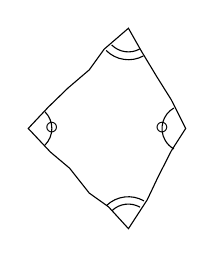
\begin{tikzpicture}[rotate=0,every node/.style={scale=1}]

\tikzstyle{MainLevee}=[decorate,decoration={random steps,amplitude=1pt,segment length=10pt}]

\coordinate (A) at (0,0);
\coordinate (B) at (45:1.8);
\coordinate (C) at (0:2);
\coordinate (D) at (-45:1.8);

\draw[MainLevee] (A) -- (B) -- (C) -- (D) --cycle;

\draw (45:0.3) arc (45:-45:0.3) node[midway]{$\circ$};
\draw (1.85,0.26) arc (119.74:240.27:0.3)node[midway]{$\circ$};

\draw (1.06,1.06) arc (-135:-61.74:0.3);
\draw (.99,.99) arc (-135:-61.74:0.4);
\draw (1.42,-1.0) arc (60.26:134:0.3);
\draw (1.47,-0.92) arc (60.26:134:0.4);

\end{tikzpicture}}, on peut affirmer que c'est un:
      \begin{ChoixQCM}{4}
      \item parallélogramme
      \item rectangle
      \item losange
      \item carré
      \end{ChoixQCM}
\begin{corrige}
     \reponseQCM{c} 
   \end{corrige}
    \end{exercice}
    
\end{GroupeQCM}
\end{QCM}

\begin{QCM}
  \begin{GroupeQCM}
\begin{exercice}
À partir du codage du quadrilatère suivant, tracé à main levée : \hspace{0.5em} \raisebox{-0.5\height}{\input{./Quadrilateres/figures/QCM_MainLevee_2}}, on peut affirmer que c'est un:
      \begin{ChoixQCM}{4}
      \item parallélogramme
      \item rectangle
      \item losange
      \item carré
      \end{ChoixQCM}
\begin{corrige}
     \reponseQCM{c} 
   \end{corrige}
    \end{exercice}

\begin{exercice}
À partir du codage du quadrilatère suivant, tracé à main levée : \hspace{0.5em} \raisebox{-0.5\height}{\input{./Quadrilateres/figures/QCM_MainLevee_3}}, on peut affirmer que c'est un:
      \begin{ChoixQCM}{4}
      \item parallélogramme
      \item rectangle
      \item losange
      \item carré
      \end{ChoixQCM}
\begin{corrige}
     \reponseQCM{c} 
   \end{corrige}
    \end{exercice}

\begin{exercice}
À partir du codage du quadrilatère suivant, tracé à main levée : \hspace{0.5em} \raisebox{-0.5\height}{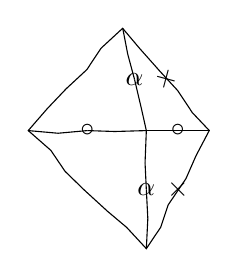
\begin{tikzpicture}[rotate=0,every node/.style={scale=1}]

\tikzstyle{MainLevee}=[decorate,decoration={random steps,amplitude=1pt,segment length=10pt}]

\coordinate (A) at (0,0);
\coordinate (B) at (1.2,1.3);
\coordinate (C) at (2.3,0);
\coordinate (D) at (1.5,-1.5);
\coordinate (O) at (1.5,0); %le centre du losange

%%%%%Les marques d'égalité de longueurs sur les diagonales :
\coordinate (A') at (0.75,0); %le milieu de la diagonale [AO]
\coordinate (B') at (1.35,0.65);
\coordinate (C') at (1.9,0);
\coordinate (D') at (1.5,-0.75);
\node at (A'){$\circ$};
\node at (B'){$\alpha$};
\node at (C'){$\circ$};
\node at (D'){$\alpha$};
%%% Les marques d'égalité de longueurs sur 2 côtés
\draw (1.75,0.65) node[rotate=30] {$\times$};
\draw (1.9,-0.75) node[rotate=0] {$\times$};

\draw[MainLevee] (A) -- (B) -- (C) -- (D) --cycle;

\draw[MainLevee] (A)--(A'); 
\draw[MainLevee] (A')--(O);
\draw[MainLevee] (B)--(B'); 
\draw[MainLevee] (B')--(O);
\draw[MainLevee] (C)--(C'); 
\draw[MainLevee] (C')--(O);
\draw[MainLevee] (D)--(D'); 
\draw[MainLevee] (D')--(O);

\end{tikzpicture}}, on peut affirmer que c'est un:
      \begin{ChoixQCM}{4}
      \item parallélogramme
      \item rectangle
      \item losange
      \item carré
      \end{ChoixQCM}
\begin{corrige}
     \reponseQCM{c} 
   \end{corrige}
    \end{exercice}

\end{GroupeQCM}
\end{QCM}

  


\TravauxPratiques % pour nous "travailler en groupe"
\input{Quadrilateres/Quadrilateres_en_groupe.tex}

\pagebreak

\recreation
\input{Quadrilateres/Quadrilateres_fin_chap.tex}


